\chapter{Evaluation}

\section{Methodology}

\section{Experimental Configuration}

Evaluation of the PBTC control strategy, Vehicle Actuated control strategy, and SCATS representation was carried out within PBTSim to measure and analyse the impact of control strategy heuristics with regards to delay and cost reductions. The experimental configuration consisted of three simulated intersection configurations, based on real-world intersections within central Wellington City; namely the intersections of Vivian Street and Victoria Street, Victoria Street and Karo Drive, and Courtney Place and Tory Street. Appedix B and C show a screenshot of each of the simulated intersection configurations within the PBTSim interface, and SCATS system respectively.

% describe the traffic configuration settings
Traffic composition was determined by a SCATS log file for each of the three evaluation intersections, SCATS log files were provided by the Wellington City Council and contained 13 hours of data logged on the 20th June, 2013. A static traffic composition configuration made up of 80\%-20\% light vehicles - heavy vehicles was used for all of the simulation runs during evaluation.

Each simulation run was repeated ten times for each of the tree controller strategies evaluated by this project, on each of the three evaluation intersections, for a total of 90 unique runs. Post-processing tools were used to report the mean and standard deviation of results for each set of repeated runs. Metrics were analysed post-experimentation using MATLAB. The set of results generated by each simulation run include the following evaluation metrics:

\begin{itemize}
\item Mean number of vehicle arrivals over each 30 second window of simulation
\item Mean delay time, cost of delay, and incurred costs of stopping for each vehicle during simulation
\item Delay time, cost of delay, and incurred costs of stopping of all vehicles over each 30 second window of simulation
\item Total delay time, cost of delay, and incurred costs of stopping for all vehicles during simulation
\end{itemize}

The Vehicle Actuated traffic control strategy was set to a fixed phase duration of 30 seconds, with minimum and maximum duration limits of 15 and 60 seconds, respectively. Each PBTSim intersection configuration was constructed to reflect the real-world configuration represented in the SCATS log files.

\begin{figure}
\centering
\begin{subfigure}{.5\textwidth}
  \centering
  \includegraphics[scale=0.35]{scats-vivian-victoria.png}
  \caption{Vivian Street-Victoria Street}
  \label{fig:sub1}
\end{subfigure}%
\begin{subfigure}{.5\textwidth}
  \centering
  \includegraphics[scale=0.35]{scats-vivian-victoria.png}
  \caption{Courtenay Place-Tory Street}
  \label{fig:sub2}
\end{subfigure}

\vspace{1cm}

\begin{subfigure}{.5\textwidth}
  \centering
  \includegraphics[scale=0.35]{scats-vivian-victoria.png}
  \caption{Karo Drive-Victoria Street}
  \label{fig:sub1}
\end{subfigure}%
\caption{The three evaluation intersections used during the experimentation procedure as represented in the SCATS system used by Wellington City Council. Screenshots were provided by City Council traffic engineers. }
\label{fig:test}
\end{figure}

\section{Traffic Flow}
\label{sec:trafficflow}

To investigate the flow of traffic through the simulation networks over the course of the simulation period, the number of vehicle arrivals was logged every 30 seconds of simulation time. The flow of traffic over a 13 hour period during a typical day can be expected to vary, and the performance of different traffic management strategies may be affected by periodic flow rates. Traffic flow within the experimentation was generated from detector data contained within the SCATS log files of each intersection. Figure ~\ref{eval:vehiclearrivalstime} shows a plot of the trend in vehicle arrivals over the simulation period for each of the evaluation intersections. Each of the three intersections show evidence of ``peak'' traffic periods, typically during the first 3 hours and last 3 hours of the evaluation window.

The Vivian-Victoria intersection has significantly higher traffic flow than the other two intersections evaluated. As the inbound link of the southern motorway, Vivian Street is an arterial link of Wellington's road network and a typical route for many Hutt Valley commuters working in the central business district (CBD). This is evidenced in ~\ref{vehiclearrivalstime:sub1}, flow recorded on the Vivian Street approach is considerably higher than Victoria Street for the majority of the evaluation window. The flow recorded at the Courtenay-Tory intersection is relatively low. As neither Courtenay Place or Tory Street are motorway approaches, the comparably lower rate of traffic flow is expected. 

The Karo-Victoria intersection shows clear evidence of morning and evening traffic peaks, with flow increasing up to the end of the evaluation period, which corresponds approximately 7pm in real-time. As Karo Drive is the entry to the northern motorway, and one of the few routes by which Hutt Valley commuters can easily leave the CBD, the end-of-day flow increase is expected. The flow rate at the Victoria Street approach to the Karo intersection remains consistently low over the entire evaluation period. From personal experience of traveling via this intersection, more than one vehicle per 30 seconds is expected on this approach which suggests the SCATS log file may be incomplete (for example, due to a failed detector) and is not reflecting the real traffic flow at that intersection. 

\begin{figure}
\centering
\begin{subfigure}{.5\textwidth}
  \centering
  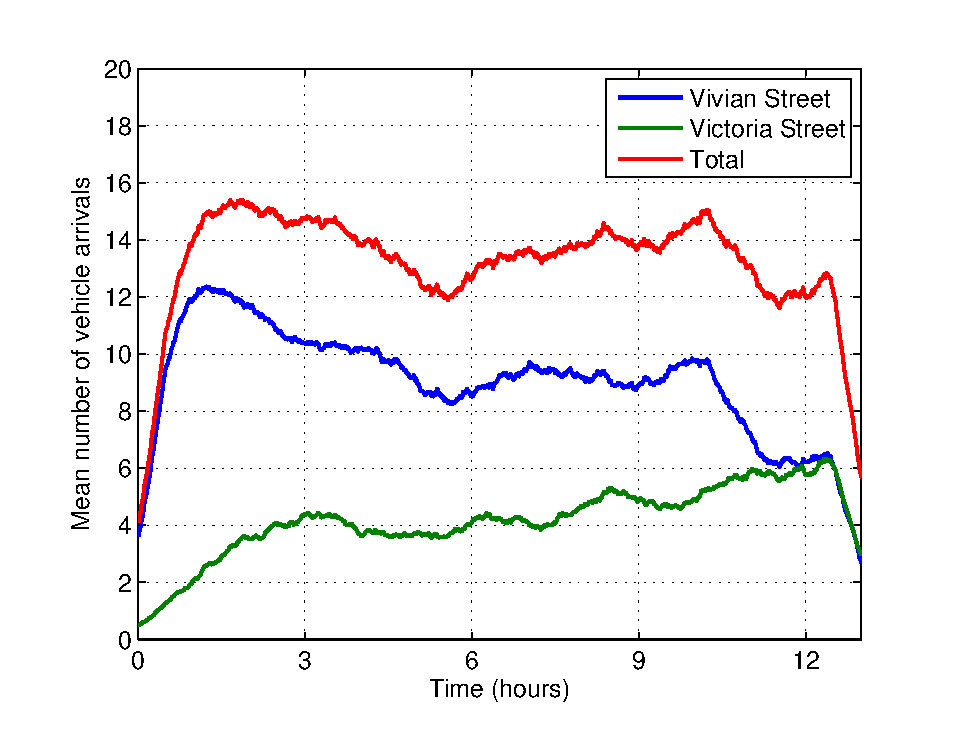
\includegraphics[scale=0.50]{vivian_victoria_num_arrivals_time.eps}
  \caption{A subfigure}
  \label{vehiclearrivalstime:sub1}
\end{subfigure}%
\begin{subfigure}{.5\textwidth}
  \centering
  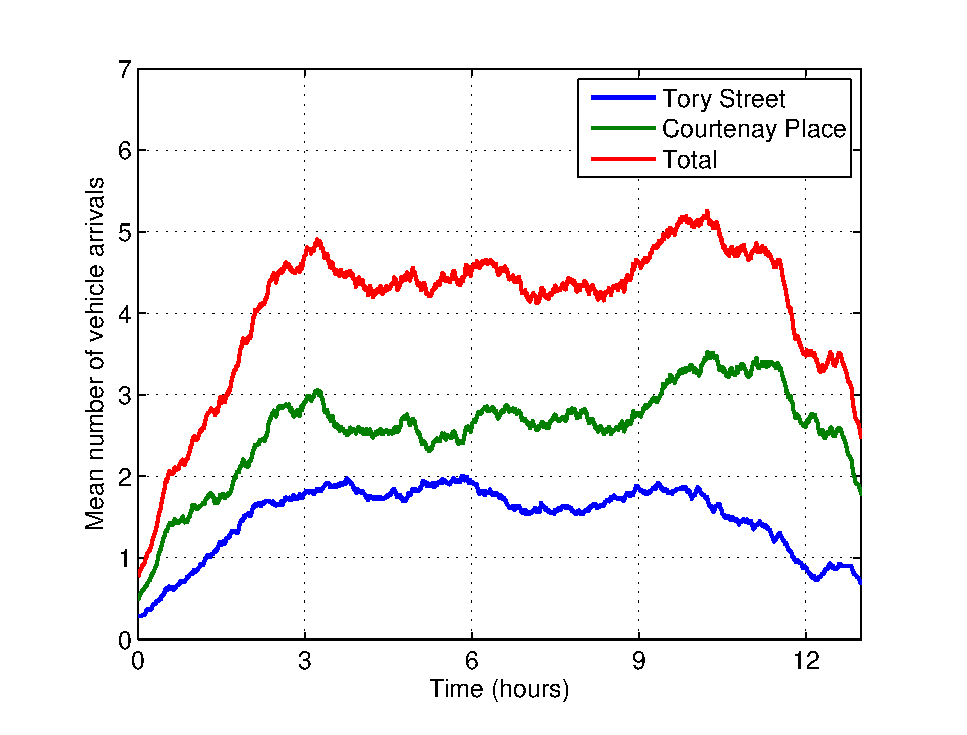
\includegraphics[scale=0.50]{courtenay_tory_num_arrivals_time.eps}
  \caption{A subfigure}
  \label{vehiclearrivalstime:sub2}
\end{subfigure}

\vspace{1cm}

\begin{subfigure}{.5\textwidth}
  \centering
  \includegraphics[scale=0.50]{karo_victoria_num_arrivals_time.eps}
  \caption{A subfigure}
  \label{vehiclearrivalstime:sub3}
\end{subfigure}%
\caption{ A plot of the trend in the mean number of vehicle arrivals per 30 seconds over the duration of the evaluation window of 13 hours for each of the evaluation intersections. The mean number of vehicle arrivals for each 30 second block is determined through use of a convolution filter to display a moving average per hour of simulation time. The filtered data effectively displays an overview of the trend of traffic flow at each hour of the evaluation window. The flow rate at all three intersections shows evidence of expected morning and evening peaks caused by worker commutes. }
\label{eval:vehiclearrivalstime}
\end{figure}

\section {Delay Time and Cost}
\label{sec:incurred_delay_cost}

Delay time and delay cost are related metrics, though the relationship is not directly proportional as the cost of delay for an individual vehicle is determined by a function of urgency as well as time. As the SCATS and Vehicle Actuated control strategies do not consider delay cost when making phase control decisions, the total time vehicles are delayed is a valuable metric for these two systems, and is a metric often raised in informal discussions related to the effectiveness of traffic lights, as the individual delay time is the most noticeable cost to road users at controlled intersections.

Figure ~\ref{eval:approaches_delay_time} shows a plot of the mean time spent delayed by individual vehicles within the experimental simulation, distributed by vehicle urgency for each of the three control strategies evaluated. The PBTC control system is able to achieve lower mean delay times across each of the three intersections, most appreciably on the intersection of Courtenay Place and Tory Street. While the performance of the Vehicle Actuated control strategy is typically the worst, the delay time recorded by the SCATS traffic controller is more comparable to the PBTC system; with the exception of the Karo-Victoria intersection where the SCATS controller consistently results in longer mean delay times across all vehicle urgencies. It is possible that the reason for the degraded SCATS performance in this area is due to an incomplete or non-representative log file for the Karo-Victoria intersection, as described in ~\ref{sec:trafficflow}. 

The difference in mean delay time between the PBTC system and SCATS or Vehicle Actuated systems appears to be more pronounced on the Karo-Victoria and Courtenay-Tory intersections. This is likely due to the lower overall flow rates recorded over the evaluation period for these two intersections. % why?

The PBTC control system also shows evidence of urgency preference within the mean delay times recorded per urgency. There is a decreasing trend in mean delay times recorded by the PBTC control system for increasing urgencies, which reflects that the PBTC control system considers cost of delay as a function of time and urgency when making control decisions. The SCATS and Vehicle Actuated control strategies do not show any evidence of this trend, as expected.
% note that there are significantly less priority 5 vehicles

\begin{figure}
\centering
\begin{subfigure}{.5\textwidth}
  \centering
  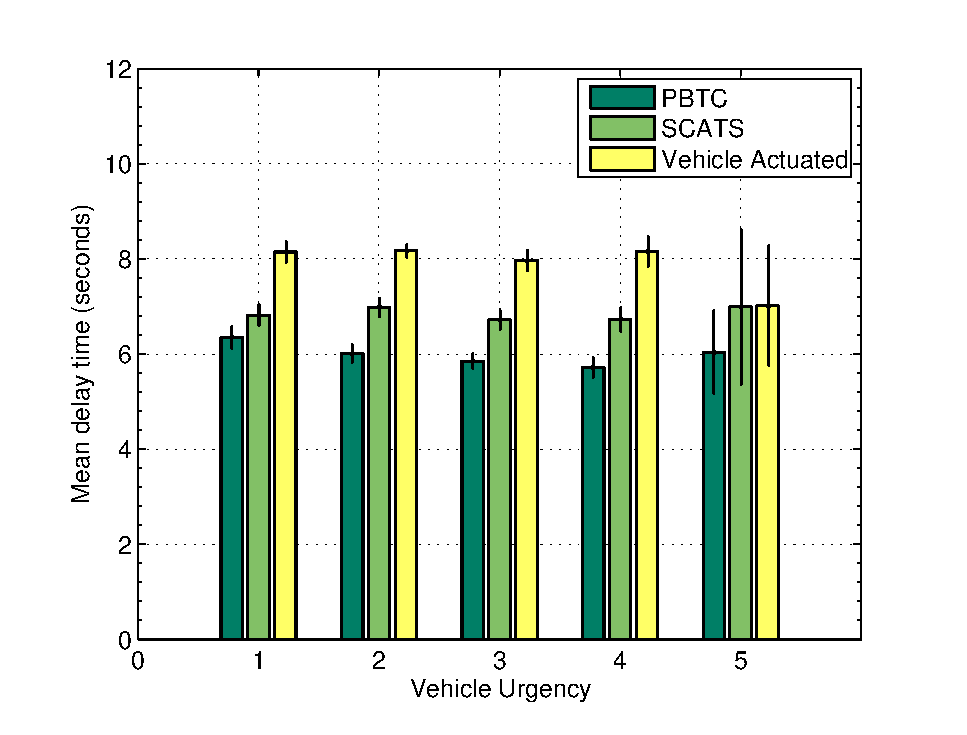
\includegraphics[scale=0.50]{vivian_victoria_approaches_delay_time.eps}
  \caption{Victoria-Vivian}
  \label{approaches_delay_time:sub1}
\end{subfigure}%
\begin{subfigure}{.5\textwidth}
  \centering
  \includegraphics[scale=0.50]{courtenay_tory_approaches_delay_time.eps}
  \caption{Courtenay-Tory}
  \label{approaches_delay_time:sub2}
\end{subfigure}

\vspace{1cm}

\begin{subfigure}{.5\textwidth}
  \centering
  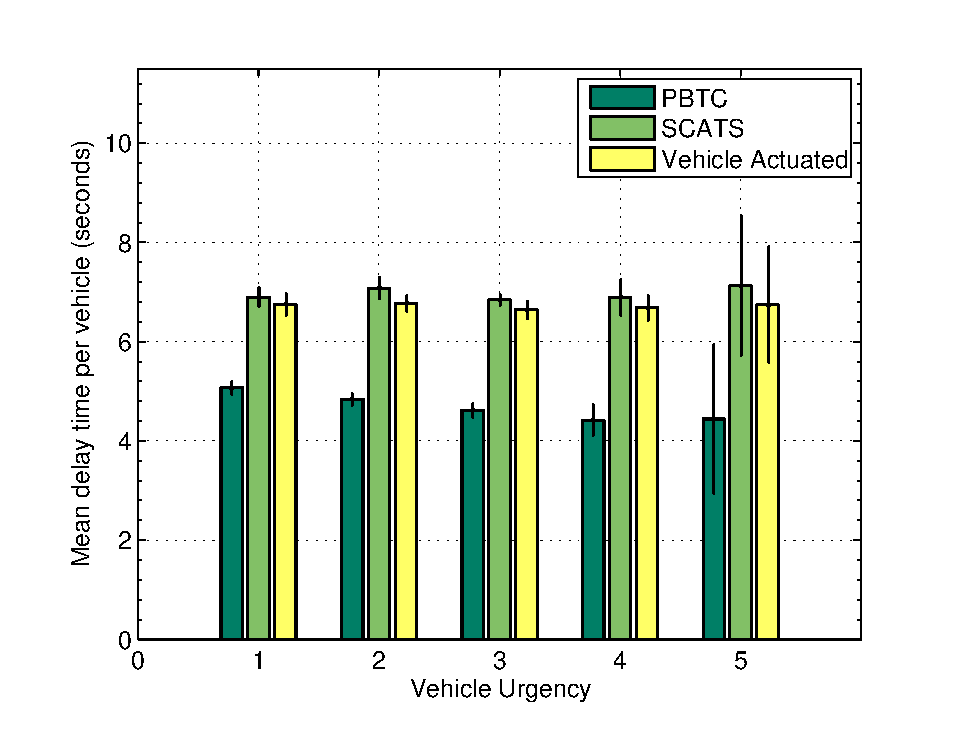
\includegraphics[scale=0.50]{karo_victoria_approaches_delay_time.eps}
  \caption{Karo-Victoria}
  \label{approaches_delay_time:sub3}
\end{subfigure}%
\caption{ A bar chart of the mean delay time, measured in seconds, for an individual vehicle in the experimental simulation for each of the three evaluation intersections. The PBTC control system outperforms SCATS and Vehicle Actuated controls over all of the dimensions.  }
\label{eval:approaches_delay_time}
\end{figure}

The PBTC system similarly outperforms the SCATS and Vehicle Actuated control strategies when considering the mean incurred cost of delay for individual vehicles within the experimental simulation. Figure ~\ref{eval:approaches_delay_cost} shows a bar chart of the delay cost, as before plotted for each of the three control strategies and grouped by vehicle urgency. 

All three control strategies display a clear trend of increasing costs as vehicle urgency increases, expected as per the design of the delay cost measure, described in ~\ref{sec:design_delay_cost}. The PBTC control system consistently results in a lower mean delay for all vehicles in each simulation run, by up to 10 cents on average. The chart ~\ref{approaches_delay_cost:sub3} shows the SCATS system consistently performs worse that both the PBTC and Vehicle Actuated strategies on the Karo Drive and Victoria Street intersection.

The standard deviation displayed on each of the charts are more significant for urgency 5 vehicles. There are two possible reasons for this increased error; firstly, there are typically less than 5\% urgency 5 vehicles in each simulation as per the urgency distribution displayed in ~\ref{urgencydistribution} and as a result the probability of delay for an urgency 5 vehicle is higher. Futhermore, as the relationship between time and delay cost for urgency 5 is greater, smaller differences in the delay time develop into larger delay costs and more significant error over a small sample.
% potentially fuck this shit

\begin{figure}
\centering
\begin{subfigure}{.5\textwidth}
  \centering
  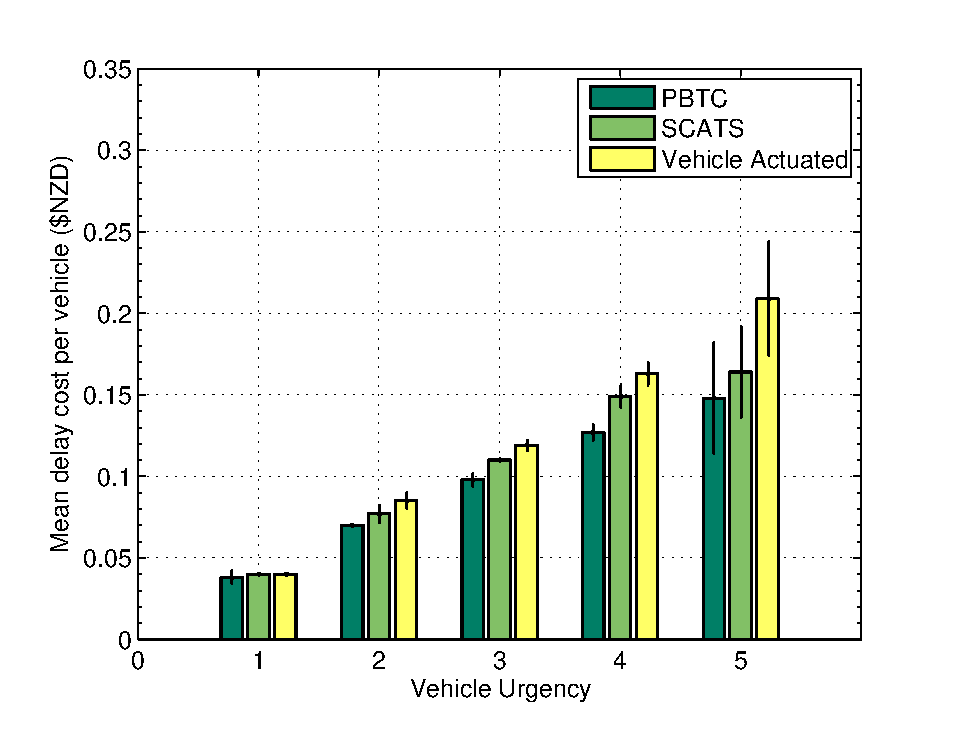
\includegraphics[scale=0.5]{vivian_victoria_approaches_delay_cost.eps}
  \caption{Vivian-Victoria}
  \label{approaches_delay_cost:sub1}
\end{subfigure}%
\begin{subfigure}{.5\textwidth}
  \centering
  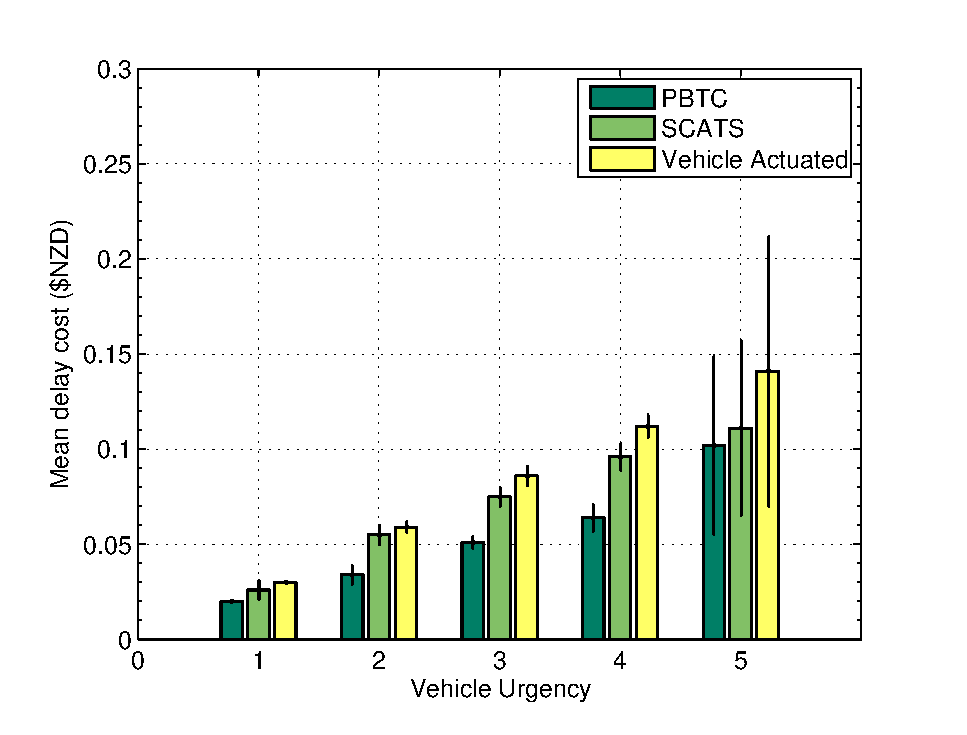
\includegraphics[scale=0.5]{courtenay_tory_approaches_delay_cost.eps}
  \caption{Courtenay-Tory}
  \label{approaches_delay_cost:sub2}
\end{subfigure}

\vspace{1cm}

\begin{subfigure}{.5\textwidth}
  \centering
  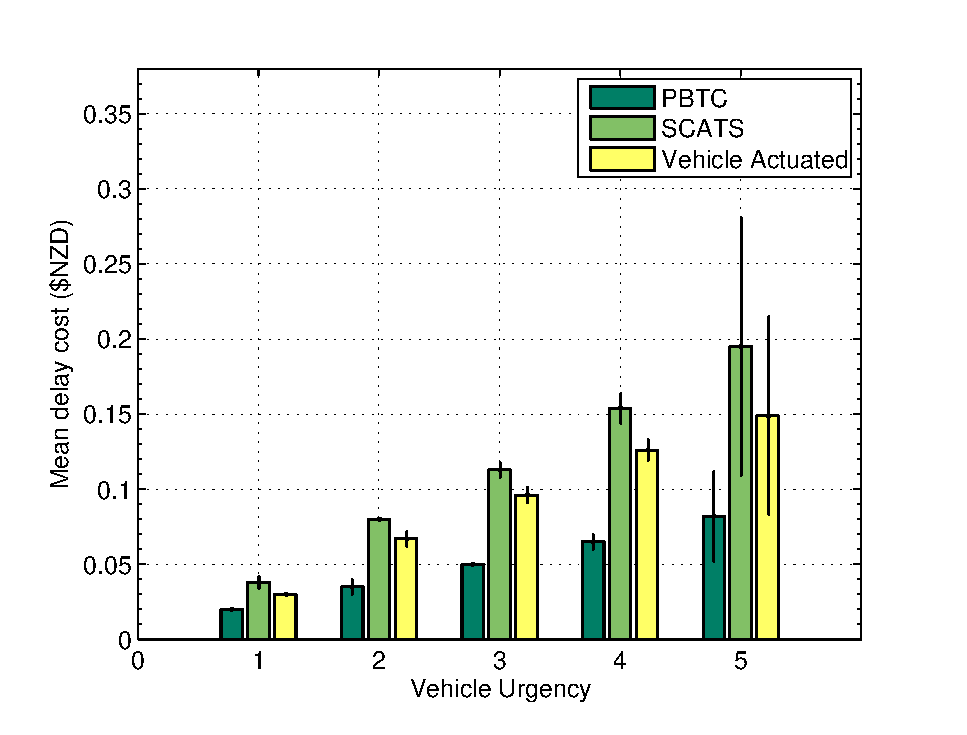
\includegraphics[scale=0.5]{karo_victoria_approaches_delay_cost.eps}
  \caption{Karo-Victoria}
  \label{approaches_delay_cost:sub3}
\end{subfigure}%
\caption{ A bar chart of the mean delay cost, in New Zealand Dollars, for an individual vehicle in the experimental simulation for each of the three evaluation intersections. The PBTC control system outperforms SCATS and Vehicle Actuated controls over all of the dimensions.  }
\label{eval:approaches_delay_cost}
\end{figure}

Further analysis of the delay cost can be made by considering the mean cost per hour of simulation time to evaluate the change in delay cost between the three systems on each intersection over the evaluation period.Figure  ~\ref{eval:delay_cost_time} shows a plot of the mean delay cost per hour of simulation time over each of the three evaluation intersections and control strategies. 

The charts presented in Figure ~\ref{eval:delay_cost_time} show a clear illustration of the difference between the adaptive PBTC and SCATS control strategies, and the non-adaptive Vehicle Actuated strategy. The mean delay cost for both the PBTC and SCATS control strategies tends to peak both in the AM period between 0 and 3 hours of simulation time and the evening period beyond 9 hours of simulation time, with a period of lower mean delay cost per hour in between. The adaptive effect is most prominently displayed on charts ~\ref{delay_cost_time:sub1} and ~\ref{delay_cost_time:sub3}, corresponding to the intersections of Victoria Street and Vivian Street and Victoria Street and Karo Drive respectively. A greater understanding of the relationship between delay cost and traffic flow can be found by comparing these results to the trend in traffic volume over the same period, as shown in Figure ~\ref{eval:vehiclearrivalstime}. The observed relationship indicates lower delay costs can be achieved by the PBTC and SCATS strategies as traffic volume decreases during the middle of the day period. This is in contrast to the results of the Vehicle Actuated system, where the mean delay cost per hour is relatively consistent over the entire period of a day, evidence of the fixed, non-adaptive nature of the Vehicle Actuated strategy.

The trend in mean delay cost per hour between the PBTC and SCATS control strategies is observed to be similar over the period of evaluation at the Vivian Street and Victoria Street intersection, as shown in chart ~\ref{delay_cost_time:sub1} . The plot of delay cost and time for the two systems follow a similar pattern, however the PBTC system achieves consistently lower delay costs across this period. This result is evidence of the incremental adaptation algorithm used by the SCATS system to adjust phase duration. SCATS and PBTC both adjust their phase times to meet the volume of demand at an intersection, though SCATS is an incremental adjustment based on near real-time flow and the PBTC system is a direct adjustment based on vehicles present in real-time, hence adjustments made by the SCATS system are slower to take effect.

In contrast, SCATS is observed to perform relatively worse than both the PBTC and Vehicle Actuated control strategies over the entire evaluation period at the intersection of Karo Drive and Victoria Street. The mean delay cost recorded by the SCATS strategy is much higher than the PBTC and Vehicle Actuated strategies between 10 and 12 hours of the evaluation period. This period is similarly explained by the incremental adaptation of the SCATS system. Traffic flow increases during this period, starting at approximately 4pm (10 hours into the simulation), corresponding with the sharp increase in mean total delay as the intersection becomes saturated and adaptive control is required to extend phase durations. After 11 hours of simulation time, mean delay costs recorded by the SCATS system actually decrease, even as the traffic flow continues to increase. This suggests that after the period of incremental adaptation, the phase times operated by SCATS eventually become optimal for the volume of traffic recorded. 

Chart ~\ref{delay_cost_time:sub3} shows that the Vehicle Actuated control strategy outperforms SCATS at the Karo Drive and Victoria Street intersection during experimentation. This result is possibly indicative that the 30-60 target-maximum durations used by the Vehicle Actuated control strategy are a good fit for this intersection over the evaluation period.

\begin{figure}
\centering
\begin{subfigure}{.5\textwidth}
  \centering
  \includegraphics[scale=0.5]{vivian_victoria_delay_cost_time.eps}
  \caption{Vivian-Victoria}
  \label{delay_cost_time:sub1}
\end{subfigure}%
\begin{subfigure}{.5\textwidth}
  \centering
  \includegraphics[scale=0.5]{courtenay_tory_delay_cost_time.eps}
  \caption{Courtenay-Tory}
  \label{delay_cost_time:sub2}
\end{subfigure}

\vspace{1cm}

\begin{subfigure}{.5\textwidth}
  \centering
  \includegraphics[scale=0.5]{karo_victoria_delay_cost_time.eps}
  \caption{Karo-Victoria}
  \label{delay_cost_time:sub3}
\end{subfigure}%
\caption{ A plot of the mean delay time per hour for each of the PBTC, SCATS, and Vehicle Actuated control strategies as applied to each of the three evaluation intersection configurations. Each plot line displays an indication of the trend in delay cost over the period of a day. The PBTC and SCATS strategies typically have lower costs between 3 and 9 hours of simulation time, which is clear evidence that these control strategies can adapt to the lower traffic volumes over this time period. The Vehicle Actuated control strategy does not adapt phase times and the mean delay cost recorded per hour is significantly higher and relatively consistent; with the exception of the Karo-Victoria intersection where the Vehicle Actuated strategy performs very well suggesting that the fixed phase times of this plan were a good fit for the traffic flow at this intersection over the evaluation period. }
\label{eval:delay_cost_time}
\end{figure}

\section{Incurred Stopping Cost}
\label{sec:incurred_stopping_cost}

The costs incurred by vehicles required to stop at a controlled intersection is another design metric of the PBTC system and as a result, analysis of the incurred stopping cost is included in this evaluation. Figure ~\ref{eval:mean_stopping_cost} shows mean stopping cost for an individual vehicle per vehicle urgency, over each of the three evaluation intersections and control strategies. 

The performance results of each strategy with regards to the mean stopping cost per vehicle urgency are mixed. There is a consistent trend of decreasing stopping cost as urgency increases over all of the control strategies for the three evaluation intersections. This trend is accordant with the distribution of vehicle urgencies shown in Table ~\ref{urgencydistribution}, as the probability of an heavy vehicle with a large cost of stopping (e.g. bus or commercial truck) having a higher urgency value is comparatively low, and not possible in the case of urgency 5. The highest recorded mean stopping costs are observed for urgency 2 vehicles, which conforms to this conclusion. %why?

Figure ~\ref{eval:mean_stopping_cost} also shows that the Vehicle Actuated control strategy performs very well with regards to reducing the mean stopping cost at all three evaluation intersections, outperforming both the SCATS and PBTC systems over a majority of the vehicle urgency values. Considered in conjunction with the mean delay time performance shown in Figure \ref{eval:mean_delay_time}, the better stopping cost performance can be explained as a byproduct of longer delay times and larger vehicle queues. Compared to freely flowing traffic, the cost of stopping individual vehicles travelling slowly in a queue is appreciably low, due to a lower instantaneous velocity at the point of stopping. As a result, an inverse relationship exists between delay cost and incurred stopping cost with respect to vehicle speed. %are you sure?

The relationship between time of day and mean stopping cost recorded per hour is shown in Figure ~\ref{eval:stopping_cost_time}. The performance of the three control strategies is relatively similar over each of the three evaluation intersections, although the mean stopping cost per hour recorded by the SCATS system appears to be consistently higher over the duration of the evaluation period. The mean stopping cost per hour measured for each of the PBTC and Vehicle Actuated control strategies is similar and varies between the three evaluation intersections. Given that the mean delay time over these periods is significantly lower for the PBTC system, the lower mean stopping cost is a benefit of the strategy itself, rather than long delay/slower traffic as is the case for the Vehicle Actuated system.
% do we need to back this up with queue stats?

\begin{figure}
\centering
\begin{subfigure}{.5\textwidth}
  \centering
  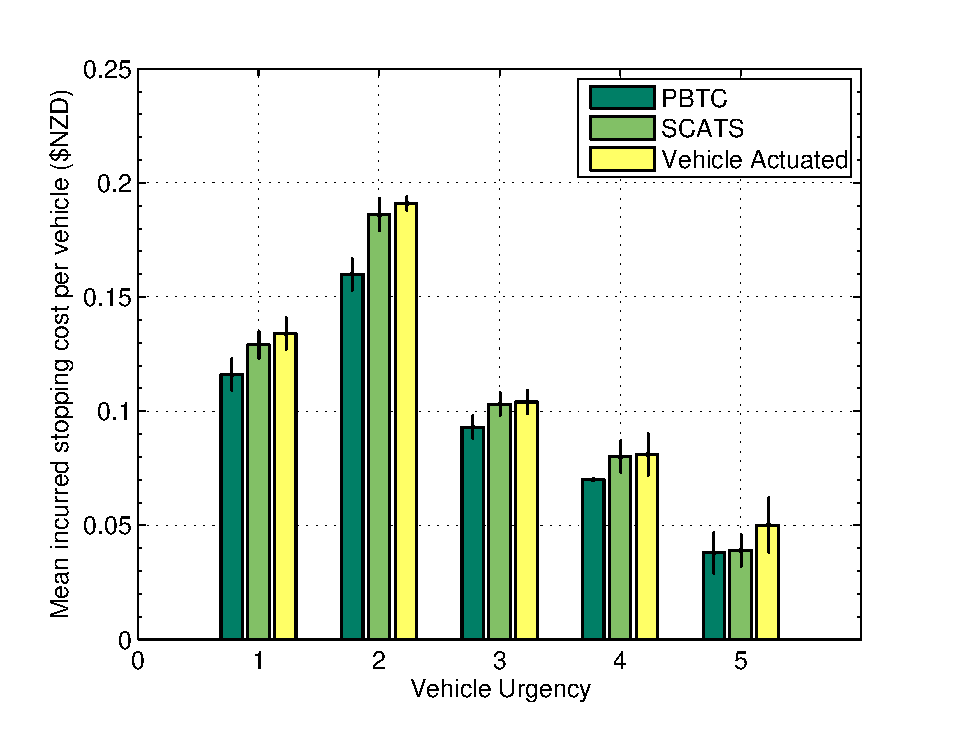
\includegraphics[scale=0.5]{vivian_victoria_approaches_stopping_cost.eps}
  \caption{Vivian-Victoria}
  \label{mean_stopping_cost:sub1}
\end{subfigure}%
\begin{subfigure}{.5\textwidth}
  \centering
  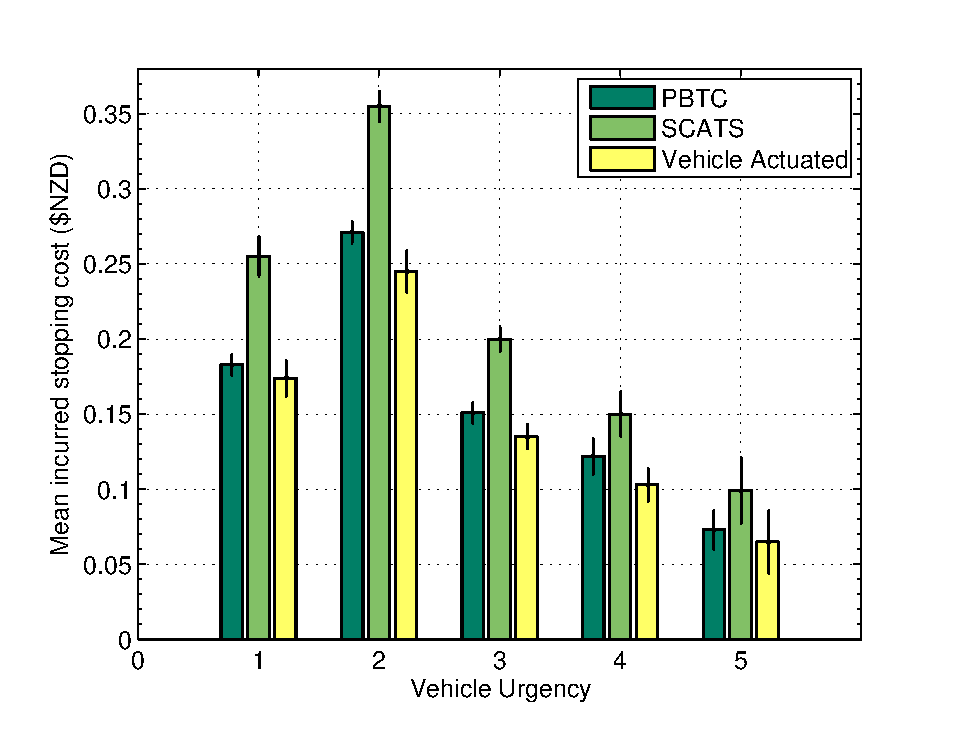
\includegraphics[scale=0.5]{courtenay_tory_approaches_stopping_cost.eps}
  \caption{Courtenay-Tory}
  \label{mean_stopping_cost:sub2}
\end{subfigure}

\vspace{1cm}

\begin{subfigure}{.5\textwidth}
  \centering
  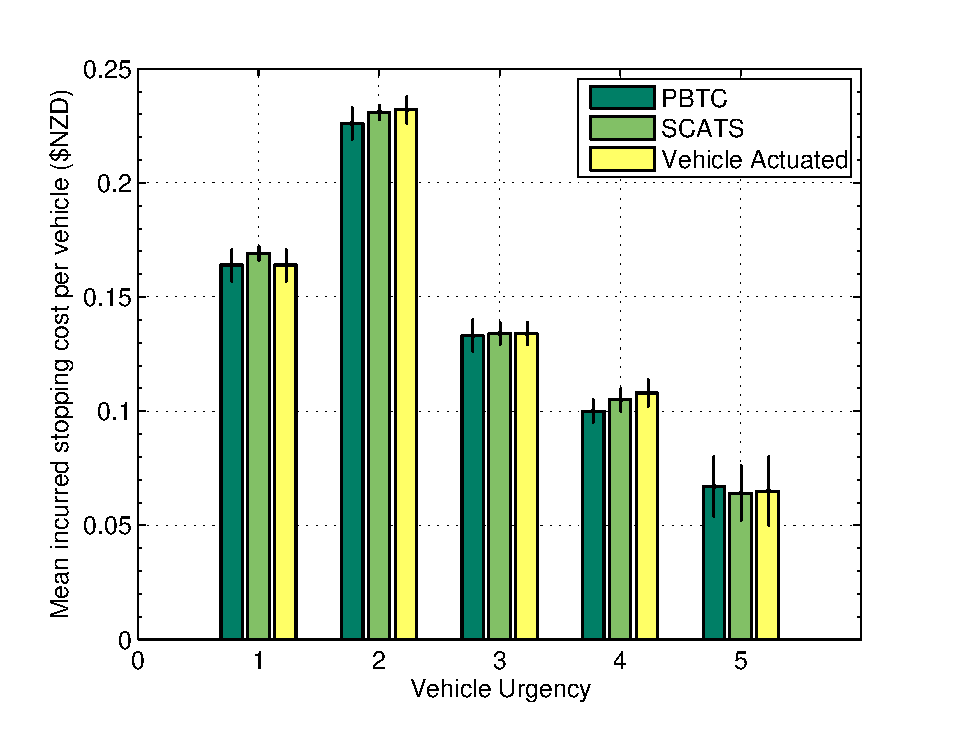
\includegraphics[scale=0.5]{karo_victoria_approaches_stopping_cost.eps}
  \caption{Karo-Victoria}
  \label{mean_stopping_cost:sub3}
\end{subfigure}%
\caption{ A bar chart of the mean stopping cost, in New Zealand Dollars, for an individual vehicle in the experimental simulation for each of the three evaluation intersections. Results of applying each control strategy are mixed, with the Vehicle Actuated strategy outperforming both SCATS and the PBTC system in a number of cases.  }
\label{eval:mean_stopping_cost}
\end{figure}

\begin{figure}
\centering
\begin{subfigure}{.5\textwidth}
  \centering
  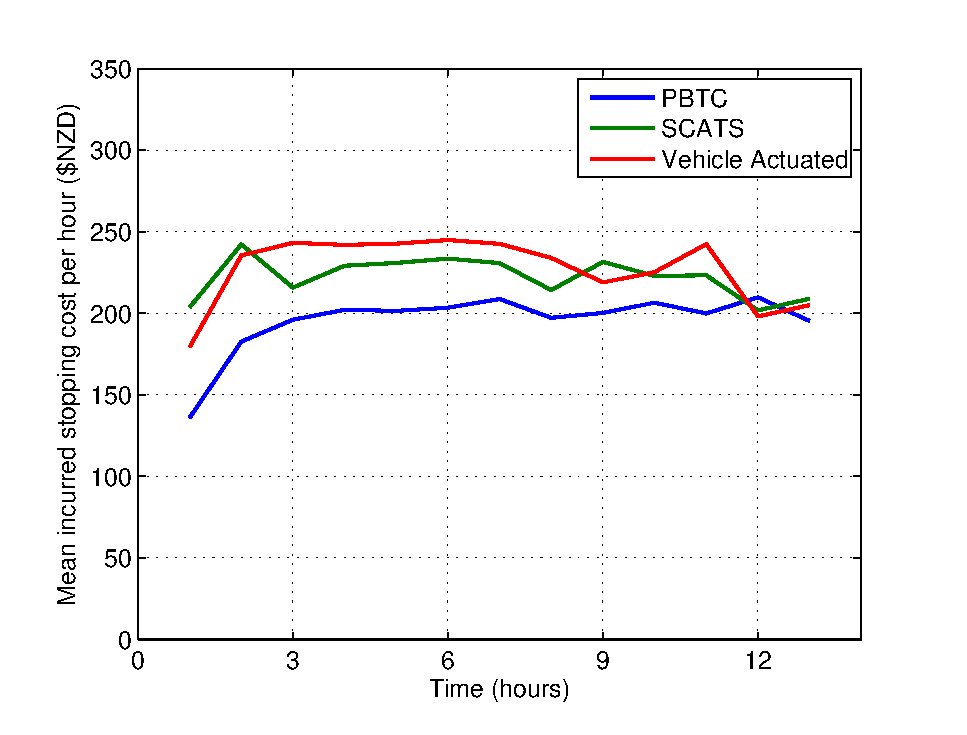
\includegraphics[scale=0.5]{vivian_victoria_stopping_cost_time.eps}
  \caption{Vivian-Victoria}
  \label{stopping_cost_time:sub1}
\end{subfigure}%
\begin{subfigure}{.5\textwidth}
  \centering
  \includegraphics[scale=0.5]{courtenay_tory_stopping_cost_time.eps}
  \caption{Courtenay-Tory}
  \label{stopping_cost_time:sub2}
\end{subfigure}

\vspace{1cm}

\begin{subfigure}{.5\textwidth}
  \centering
  \includegraphics[scale=0.5]{karo_victoria_stopping_cost_time.eps}
  \caption{Karo-Victoria}
  \label{stopping_cost_time:sub3}
\end{subfigure}%
\caption{ A plot of the mean incurred stopping cost per hour for each of the PBTC, SCATS, and Vehicle Actuated control strategies as applied to each of the three evaluation intersection configurations. Each plot line displays an indication of the trend in stopping cost over the period of a day.  }
\label{eval:stopping_cost_time }
\end{figure}

\section{Overall Incurred Costs}

The overall incurred cost of operation over the evaluation period is an important metric as the primary goal of the PBTC system is to reduce the overall operation costs by including consideration of individual vehicle costs in traffic control  decisions. Figure ~\ref{eval:total_cost} shows the mean and standard deviation of the total overall costs measured for 10 simulation runs on each of the simulated intersections. 

\begin{figure}
\centering
\begin{subfigure}{.5\textwidth}
  \centering
  \includegraphics[scale=0.5]{vivian_victoria_approaches_total_cost.eps}
  \caption{Vivian-Victoria}
  \label{total_cost:sub1}
\end{subfigure}%
\begin{subfigure}{.5\textwidth}
  \centering
  \includegraphics[scale=0.5]{courtenay_tory_approaches_total_cost.eps}
  \caption{Courtenay-Tory}
  \label{total_cost:sub2}
\end{subfigure}

\vspace{1cm}

\begin{subfigure}{.5\textwidth}
  \centering
  \includegraphics[scale=0.5]{karo_victoria_approaches_total_cost.eps}
  \caption{Karo-Victoria}
  \label{total_cost:sub3}
\end{subfigure}%
\caption{The intersection of Vivian Street and Victoria Street in Te Aro, Wellington City, as viewed in the SCATS management application in use by Wellington City Council. }
\label{eval:total_cost}
\end{figure}

The PBTC control strategy achieves the lowest mean total cost over all three simulated intersections, with a 17\% to 32.5\% reduction in overall costs compared to the SCATS control strategy, and 7.5\% to 11.3\% when compared to the Vehicle Actuated strategy. This result is supported by the results of the previous sections, where the PBTC control system is able to achieve the lowest delay time and cost and relatively low incurred stopping costs, for all of the simulated intersections. 

These results also show that the Vehicle Actuated control strategy outperforms SCATS with respect to the mean total cost for the evaluation period across all of the simulation intersections. This result is not unexpected, as the SCATS system inherently aims to reduce the total delay cost at an intersection. The results of sections ~\ref{sec:incurred_delay_cost}~ and \ref{sec:incurred_stopping_cost} clearly show that the stopping cost is a more significant factor that accounts for a larger proportion of the overall costs incurred during intersection operation. The poor performance of the Vehicle Actuated strategy with respect to delay time creates long, slow-moving vehicle queues; where stopping the queue does not incur significant stopping cost for each individual vehicle and as a result the overall cost is observed to be lower than that of SCATS. Although this result appears positive for the Vehicle Actuated strategy, in practice the long delay times are undesirable and increase the potential for queues to limit the throughput of the infrastructure to the point where the network reaches a ``gridlock'' preventing queues from clearing. 

The results presented in this experimental evaluation support the notion of a cost tradeoff between stopping a currently flowing traffic approach and delaying all other competing approaches, the design basis of the PBTC system. To analyse how each of the strategies evaluated balances these cost values, Figure ~\ref{eval:cycle_durations} shows a plot of the mean cycle duration over a ten-cycle period for each of the three control strategies over the period of each simulation run. 

\begin{table}[]
\begin{center}
\begin{tabular}{llrlrlr}
\toprule
 & \multicolumn{2}{c}{Vivian-Victoria} & \multicolumn{2}{c}{Courtenay-Tory} & \multicolumn{2}{c}{Karo-Victoria} \\
 \cmidrule(lr){2-3}
 \cmidrule(lr){4-5}
  \cmidrule(lr){6-7}
Strategy &  Total Cost & \Delta\% & Total Cost & \Delta\% & Total Cost & \Delta\% \\
\midrule
PBTC & 2544.05 (\pm 30.4) &  & 1716.43 (\pm 28.0) & & 2200.55 (\pm 43.6) & \\
SCATS & 2977.81 (\pm 66.4) & +17.0\% & 2274.18 (\pm 32.1) & +32.5\%  & 2820.03 (\pm 45.4) & +28.1\% \\ 
VA & 2762.82 (\pm 40.5) & +8.6\% & 1845.59 (\pm 32.9) & +7.5\% & 2448.80 (\pm 38.7) & +11.3\% \\
\bottomrule
\end{tabular}
\end{center}
\caption{ Mean total cost (NZD) of ten simulation runs, and percentage difference relative to the performance of the PBTC system for each of the three control strategies and intersection examples used in evaluation. Mean total cost error is the standard deviation of the mean total cost for ten simulation runs. The PBTC control system achieves between 17.0\% to 32.5\% reduction of the total costs of operation over the 13-hour evaluation period. }
	\label{urgencydistribution}
\end{table}

\begin{figure}
\centering
\begin{subfigure}{.5\textwidth}
  \centering
  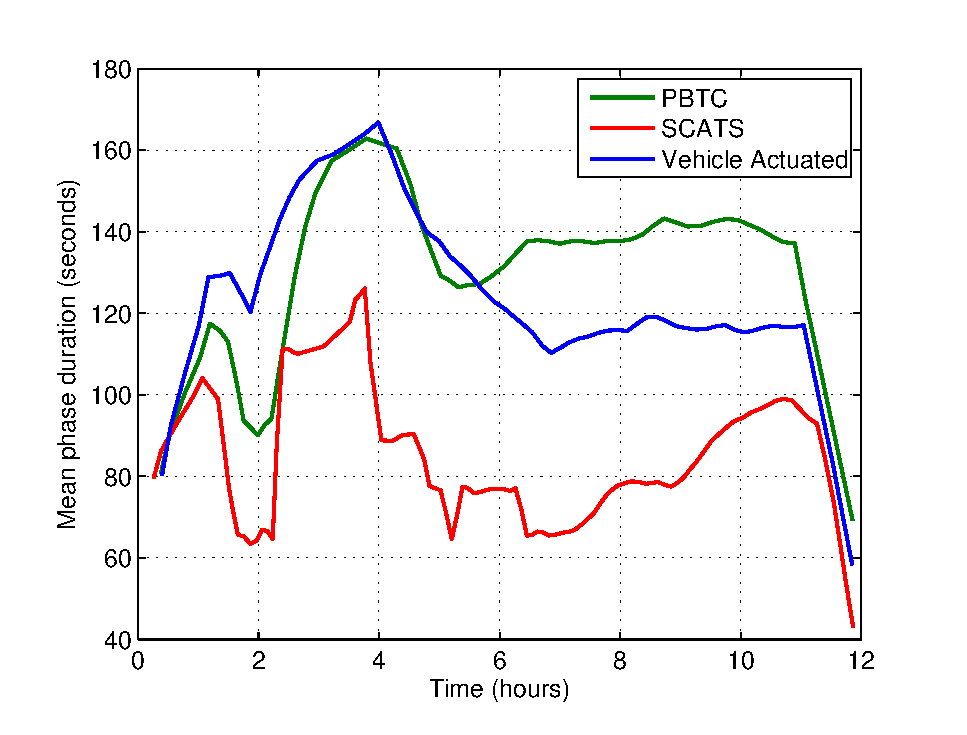
\includegraphics[scale=0.5]{vivian_victoria_cycle_durations.eps}
  \caption{Vivian-Victoria}
  \label{cycle_durations:sub1}
\end{subfigure}%
\begin{subfigure}{.5\textwidth}
  \centering
  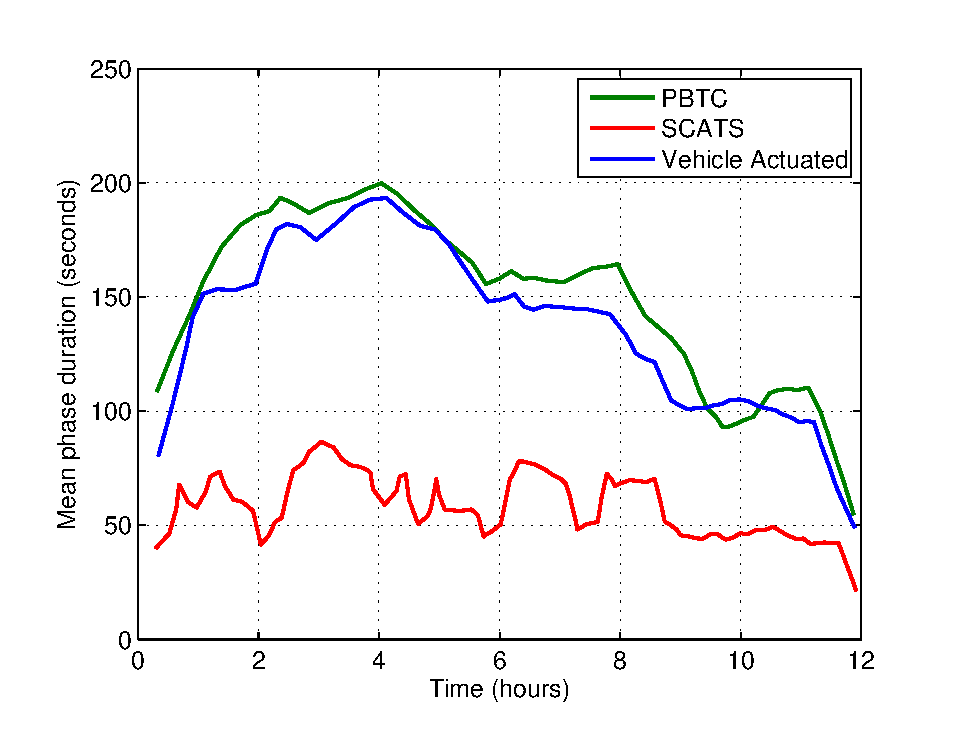
\includegraphics[scale=0.5]{courtenay_tory_cycle_durations.eps}
  \caption{Courtenay-Tory}
  \label{cycle_durations:sub2}
\end{subfigure}

\vspace{1cm}

\begin{subfigure}{.5\textwidth}
  \centering
  \includegraphics[scale=0.5]{karo_victoria_cycle_durations.eps}
  \caption{Karo-Victoria}
  \label{cycle_durations:sub3}
\end{subfigure}%
\caption{ A plot of the mean cycle duration in seconds for each of the PBTC, SCATS, and Vehicle Actuated control strategies over each of the simulated intersections.   }
\label{eval:cycle_durations}
\end{figure}




